\chapter{Testing}\label{ch:testing}
In order to validate that the compiler is correct, unit, integration, and acceptance testing is conducted and explained in this chapter. Furthermore, a user testing plan is described.\\
Selected tests are displayed in this chapter, and the rest are displayed in appendix \ref{appendix:Testing}.

\section{Testing of the \lang compiler} \label{sec:test_strat}
The testing is conducted by using the Arrange, Act \& Assert (AAA) testing pattern. This is a pattern that helps make tests clear and understandable because of the separation between the setup, execution, and verification parts of the test. The Arrange section initializes objects and variables passed to the method being tested. The Act section invokes the said method with the arranged parameters. Lastly, the Assert section is the one that clarifies if the test is successful or not, by setting one or more conditions that, if true, means that the test is successful \cite{unittestbasics}. As a metric to get an understanding of which parts of the program are tested and which are not, a code coverage overview is made. As shown in figure \ref{fig:code_coverage}, not all of the code is tested. This is due to time restraint or the code not being important to the compiler. This is for example the \textit{prettyPrint()} function in the \textit{BuildASTVistior} class, as it only acts as a visualization under development. The setup of testing is done by creating a whole new separate project inside the same solution in visual studio. That way we can access the necessary methods that have to be tested.\\
All tests are accessible in the project repository in GitHub \cite{p4-project-rep}.

\begin{figure}[H]
    \begin{center}
        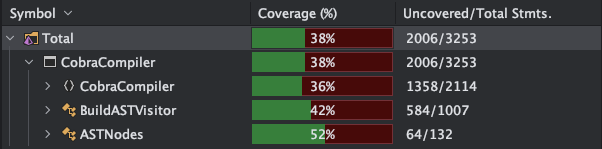
\includegraphics[width=0.8\textwidth]{Files/Billeder: Test/code_coverage.png}
    \end{center}
    \caption{Code coverage}
    \label{fig:code_coverage}
\end{figure}

\section{Unit Test}
The first level of testing conducted is unit testing. Unit testing is the smallest testable part of an application and the purpose of unit testing is to separate modules from their dependencies and test individual methods. The framework we use for testing is NUnit \cite{nunit}, which is a unit-testing framework for all .Net languages that support the AAA testing pattern. As mentioned in section \ref{sec:test_strat}, only some code is unit tested. This is due to most of the \lang compiler consisting of visitor patterns which are easier to test using integration testing because of the number of functions integrated with each other. This is shown in section \ref{sec:intergationTest}.\\

An example of a unit test can be seen in listing \ref{list:symbol_newscope_pushtostack}. The function being tested is \textit{NewScope()} by asserting if a new scope had been added to the stack of scopes in the symbol table. The Arrange block creates new instances of \textit{SymbolTable()} and \textit{BlockNode()} on lines 57-58. In the Act stage, \textit{NewScope()} in the symbol table is called and the block node is passed as an argument to the method. This happens on line 61. This should open a new scope containing the given block node. To test that \textit{NewScope()} did push this new scope to the stack, we test that our \textit{symbolTable.\_stackScopes} contains one scope on line 64. This will return true if \textit{NewScope()} pushes a new scope onto the stack. We also test that the stack contains a scope with a block that is equal to \textit{blockNode} on line 65. When running these tests, a green mark is displayed if all of the Assert methods return true. If this is the case, it can be concluded that these unit tests are successful, and in this case, the \textit{NewScope()} method in listing \ref{list:symbol_newscope_pushtostack} works as expected.

\begin{lstlisting}[language = csharp, firstnumber=53, label={list:symbol_newscope_pushtostack}, caption=Unit test of the NewScope() method that creates a new scope and tests if it pushes this scope to the stack - PEAKCompilerTesting / SymbolTableUnitTest.cs]
[Test]
public void NewScope_PushesScopeToStackScopes()
{
    // Arrange
    var symbolTable = new SymbolTable(new ErrorHandler());
    var blockNode = new ASTNodes.BlockNode();

    // Act
    symbolTable.NewScope(blockNode);

    // Assert
    That(symbolTable._stackScopes, Has.Count.EqualTo(1));
    That(symbolTable._stackScopes.Peek().Block, Is.EqualTo(blockNode));
}
\end{lstlisting}

\section{Integration Test} \label{sec:intergationTest}
As unit testing is for verifying the individual performance of modules and methods, integration testing has the purpose of verifying that they still exhibit the expected behavior as a group. This means that individual modules are combined and tested as a group to evaluate the compliance of the compiler. This section will test how the lexer, parser, AST builder, code generator, and so on work in conjunction.\\

The code in listing \ref{list:symbol_lookup_unittest} is the integration test for \textit{lookup()} in the symbol table. The \textit{SymbolTableintegrationTest} class contains all integration tests associated with the symbol table. The integration test in listing \ref{list:symbol_lookup_unittest} starts by creating a new instance of the \textit{SymbolTable} on line 9. Then a \textit{BlockNode} named \textit{blockNode1} gets instantiated on line 10. Then \textit{NewScope()} in the symbol table is called with \textit{blockNode1} as its argument on line 11. The \textit{Insert()} method is called twice to insert \textit{"x"} and \textit{"y"} in the current scope, which is the one belonging to \textit{blockNode1}. This happens on line 12-13. This concludes the Arrange stage. In the Act stage, we call \textit{Lookup()} in the symbol table three times on line 16-18. This looks for \textit{"x"}, \textit{"y"}, and \textit{"z"} in the current scope. These methods return objects of type \textit{Symbol} which contains a name, reference, and type. These symbols are checked in the assert section to see if the names of the symbols match what is expected. \textit{"z"} is not inserted in the symbol table and should therefore return \textit{null}. These asserts happen on line 21-23.\\

\begin{lstlisting}[language = csharp, firstnumber=3, label={list:symbol_lookup_unittest}, caption=Integration test of the lookup method from the symbol table - PEAKCompilerTesting / SymbolTableIntegrationTest.cs]
public class SymbolTableIntegrationTest
{
    [Test]
    public void Lookup_ReturnsCorrectSymbol()
    {
        // Arrange
        var symbolTable = new SymbolTable(new ErrorHandler());
        var blockNode1 = new ASTNodes.BlockNode();
        symbolTable.NewScope(blockNode1);
        symbolTable.Insert("x", ASTNodes.TypeEnum.text, blockNode1);
        symbolTable.Insert("y", ASTNodes.TypeEnum.text, blockNode1);
        
        // Act
        var result1 = symbolTable.Lookup("x", blockNode1);
        var result2 = symbolTable.Lookup("y", blockNode1);
        var result3 = symbolTable.Lookup("z", blockNode1);

        // Assert
        Assert.That(result1.Name, Is.EqualTo("x"));
        Assert.That(result2.Name, Is.EqualTo("y"));
        Assert.That(result3, Is.Null);
    }
}
\end{lstlisting}

\noindent The second integration test shown in listing 
\ref{list:EmitterTest} is a visit function for visiting the program node in the code generation phase. Code generation is done by the \textit{Emitter} class, which goes through the program, using the visitor pattern, and converts the program into the equivalent version in C. The C version is kept in a string builder which can then be tested. A string of \lang code that is used for testing the emitter can be seen on line 85. The string declares a number variable \textit{x} to the value \textit{10}. All the phases that lead up to the code generation, are then run in the rest of the arrange section. In the Act section, the function which visits the root node in the emitter is run on line 89. The generated C code is returned to a variable \textit{sb} of type string builder. The expected string of C code is built on line 91-95, and are then tested for equivalence in the Assert section on line 98. The goal of this test is to make sure, the emitter returns the correct C program as a string.\\

\begin{lstlisting}[language = csharp, firstnumber=82, label={list:EmitterTest}, caption=Integration test of the Emitter class used in the code generation phase - PEAKCompilerTesting / EmitterTest.cs]
public void EmitterVarDec()
{
    // Arrange
    var exprText = "number x = 10;";
    ...
    
    // Act
    StringBuilder sb = new Emitter(st).Visit((ASTNodes.ProgramNode)ast);

    String testString = "#include <stdio.h>\n#include <stdlib.h>\n#include <string.h>\nchar* concat(const char *str1, const char *str2) " 
        + 
        ...
        +
    "return curr_node->value;\n}\nvoid main(){\nint x = 10;\n}\n";

    // Assert
    Assert.That(sb.ToString(), Is.EqualTo(testString));
}
\end{lstlisting}

\section{Acceptance Test} \label{AccTest}
This section will cover the acceptance tests made to determine if the \lang compiler generates the correct target code. This is done by running a number of \lang code examples through our compiler and checking whether the resulting programs are as expected. These tests are based on the beginner exercises explained in section \ref{requirements}. If the code compiles correctly to C without errors, the C code is then compiled and run in order to see if the terminal prints the expected results. Furthermore, the generated C program is inspected to ensure it is correctly translated.\\ 
Each test contains the code written in \lang, then the code compiled to C, and finally the result of compiling and executing the C code.

%\cite{miller2001acceptance}

\subsection{Code Example: Scope test} \label{test_scopee}
The code example in listing \ref{list:acceptance_test_scope} is used to show that the scope rules defined in chapter \ref{ch:language_design} work as intended in \lang. In the example, a number \textit{y} is declared in the outer scope on line 1 with the value \textit{10}. Then \textit{print()} is declared which prints \textit{y} using \textit{output()} on line 2-5. \textit{output()} is then called with \textit{y} in the outer scope on line 6. In the if statement with condition \textit{true}, \textit{print()} is called followed by \textit{y} being outputted on lines 7-10. Then \textit{y} is redeclared with value \textit{12} on line 11 and then \textit{print()} is called, followed by \textit{y} being outputted on line 12-13. The \textit{print()} functions declaration can only access the global \textit{y} with value \textit{10} and should therefore output \textit{10},  while the \textit{output()} on line 13 should print \textit{12}. After the if-statement the \textit{print()} and \textit{output()} functions should output \textit{10} on line 15-16. The result can be seen in figure \ref{figure:scope_result}.

\newpage
\subsubsection{Source Code in \lang:}
\begin{lstlisting}[language = scriptkid, firstnumber=1, label={list:acceptance_test_scope}, caption=Acceptance test scope code examples]
number y = 10; 
function print() return nothing 
{ 
    call output(y); 
} 
call output(y);
if(true) 
{	 
    call print(); 
    call output(y);
    number y = 12; 
    call print(); 
    call output(y);
}
call print();
call output(y);
\end{lstlisting}

\subsubsection{Target code in C:}
In listing \ref{list:acceptance_test_scope_output}, the generated C code from the scope test program is displayed. From lines 1-4, the void function \textit{print()} is defined. It takes a parameter \textit{y}, which is then outputted in the function. \\
When first creating this test, an issue arose which was caused by translating the scope rules defined in \lang's semantics to code written in C. This issue was caused by the differences in starting points for \lang and C. In both C and \lang, functions can only be declared in the global scope. However, unlike in \lang where the starting point is placed at the first line of code, C uses the function \textit{main()} as its starting point. This results in a problem when declaring functions in \lang, which is addressed in section \ref{emitter:functions}. \\
The original version is identical to the output shown in listing \ref{list:acceptance_test_scope_output} except in the original, where nothing is used to distinguish between the first and second declarations of the variable \textit{y}. The \textit{print\_()} function on line 13 referenced the \textit{y} variable initialized on line 12, but in reality, it should have referenced the \textit{y} on line 6.\\
This issue required a fix to help distinguish between declared variables of the same name. The fix is described in section \ref{Implementation:SymbolTableScopeFix}. The code snippet shown in listing \ref{list:acceptance_test_scope_output} displays the resulting C code after the fix, and correlates with the program in \lang. The result when executing the code can be seen in figure \ref{figure:scope_result}.

\newpage
\begin{lstlisting}[language = C, captionpos=b, firstnumber=1, label={list:acceptance_test_scope_output}, caption=Acceptance test scope code examples in C]
void print_(int y)
{
    printf("%d\n", y);
}
void main() {
    int y = 10;
    printf("%d\n", y);
    if (1)
    {
        print_(y);
        printf("%d\n", y);
        int y_ = 12;
        print_(y);
        printf("%d\n", y_);
    }
    print_(y);
    printf("%d\n", y);
}
\end{lstlisting}

\subsubsection{Result:}
\begin{figure}[H] 
    \begin{center}
        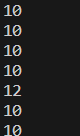
\includegraphics[width=0.20\textwidth]{Files/Billeder: Appendix/Scopetest.png}
    \end{center}
    \caption{The result for the scope code example}
    \label{figure:scope_result}
\end{figure}

\newpage
\subsection{Code Example: Update of variables} \label{test_UpdateVar}

The code example in listing \ref{list:acceptance_test_input_update_test} is used to show that declaration and re-assignment of an existing variable works as intended. First, multiple different variables of different types are declared on lines 1-3, and \textit{n} is then outputted on line 5. Afterward, the user is prompted for a new input for \textit{n} on line 7. This new value of \textit{n} is then outputted on line 9. A couple of examples of comments can be seen on lines 10-11, which are ignored when compiling to C. The new \textit{n} should overwrite the original value of \textit{n}.

\subsubsection{Source Code in \lang:} \label{}
\begin{lstlisting}[language = scriptkid, firstnumber=1, label={list:acceptance_test_input_update_test}, caption=Acceptance test update of variables with input code examples]
number n = 123;
text t = "test";  
decimal d = 0.20123123947342375;  
call output("Previous value is "); 
call output (n); 
call output(". Please input a new number");
n = call number input();  
call output("New value is "); 
call output(n);  
comment: This is a comment;
comment: This is also a comment;  
\end{lstlisting}

The C code in listing \ref{list:acceptance_test_input_update_text_output} corresponds to what is expected. First, the three different variables are declared on lines 3-5, whereafter three lines are printed to the console on lines 6-8. Next, \textit{input()} is called. The input function is a custom helper function that is added to the emitter. It takes in a format and the variable size, scans a user input, and returns it. The \textit{input()} function returns a void pointer, which needs to be cast to the correct pointer type and dereferenced to get the value. This can be seen on line 9. Note that the decimal value in listing \ref{list:acceptance_test_input_update_test} is rounded up when compiling to C. This is because float only being able to contain 7 decimals \cite{Float7Dec}. This was first discovered when running the code example in listing \ref{list:acceptance_test_input_update_text_output}. This is touched upon in the discussion section \ref{Diss:CompilerRev}. The result when executing the code is displayed in figure \ref{figure:input_update_result}.

\subsubsection{Target code in C:}
\begin{lstlisting}[language = C, firstnumber=1, captionpos=b, label={list:acceptance_test_input_update_text_output}, caption=Acceptance test update of variables with input code examples in C]
void main()
{
int n = 123;
char * t = "test";
float d = 0.20123124;
printf("%s\n", "Previous value is ");
printf("%d\n", n);
printf("%s\n", ". Please input a new number");
n = *(int *)input("%d", sizeof(int));
printf("%s\n", "New value is ");
printf("%d\n", n);
}
\end{lstlisting}

\subsubsection{Result:}
\begin{figure}[H] 
    \begin{center}
        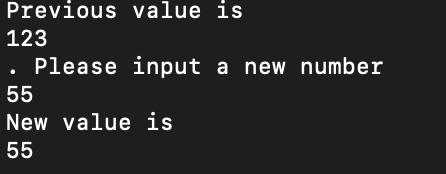
\includegraphics[width=0.40\textwidth]{Files/Billeder: Appendix/InputUpdate.png}
    \end{center}
    \caption{The result for the variable update code example}
    \label{figure:input_update_result}
\end{figure}

Along with these examples, some other acceptance tests are also made. These can be seen in section \ref{Appendix:acceptance_test} in the appendix. A short description of these examples can be seen below:

\begin{itemize}
    \item \textbf{Insertion-Sort:} This code example initializes a list of numbers and prints them. Afterward, this list is sorted using the 'SortNumberList()' which uses the insertion-sort algorithm. The new sorted list is then also printed.
    \item \textbf{Time-Conversion:} This code takes a number of seconds as input. By using division and a function 'mod()', which calculates modulo, it calculates how many weeks, days, hours, and minutes these seconds are equivalent to. These values are then printed.
    \item \textbf{GCD calculator:} This code calculates the 'greatest-common-divisor' of two numbers. this code includes 'GetMax()', 'GetMin()' and 'mod()'. In case the given input is wrong, the user is asked once again for an input. After printing GCD, the code gives the user the opportunity to write two new numbers.
    \item \textbf{Input Repeat:} This example declares a function called 'StartFunction()'. This function has a while-loop which runs while a boolean value is true. In the loop, the user is prompted and asked to write "start" to begin. The user is then asked to write how many times a message should be repeated. A message saying "This is a repeated message" is then repeated to the number requested by the user. Afterward, the user is prompted to write 'start' again.
    \item \textbf{Triangle Area:} This example declares a function 'triArea()' which calculates the area of a triangle. This function is then called and printed four times, all with different inputs.
    \item \textbf{Mathematical Expressions:} This example tests that all the mathematical expressions included in \lang works as intended. This is done by declaring variables and using the infix mathematical expressions on the variables.
    \item \textbf{Missing semi error:} This code example is used to test if the correct error is being output when the code is missing a ";".
    \item \textbf{Wrong type:} This code example tests the output message for when an incorrect type has been used.
    \item \textbf{String concatenation:} This code example is used to test for string concatenation. this is done by creating a text variable and using the infix operator "+" between two strings, and afterward outputting the variable.
    \item \textbf{Zero division:} This code example is used to make sure that division by zero is not possible in \lang and that it gives the correct output in the terminal.
\end{itemize}

\subsection{User Testing}\label{usertesting}
In order to test and get feedback on whether or not \lang has succeeded to become a beginner-friendly programming language, a user testing plan is produced.
First up, the tester has to be exposed to a number of small programs written in two different languages, one should be \lang and the other should be in a non-beginner-friendly language as mentioned in section \ref{SelectionLang}. The purpose of this is to test the readability of \lang, by having the tester look through these programs and write down what the tester thinks the programs do.\\


%The last part of the user test will cover the usage of \lang. The tester have to be introduced to \lang functionality, and the basics of it, and then write a specific program. Afterward, you could then show the tester another language and ask them to write the same program in that language. That way, we could see whether or not \lang is more intuitive to learn syntax-wise than a language for more experienced programmers. This type of test would suit more experienced beginner programmers than a beginner program that has not programmed before, as you would need the basic foundation of how to program.\\

Second, the user test will cover the usage of \lang. The tester has to be introduced to \lang functionality, and the basics of it, to be able to write a basic beginner programming exercise, like those explained in section \ref{requirements}, that the requirement for \lang is build upon. In this test, we will observe if the tester has problems writing code in \lang. This is done to test whether or not it is intuitive to learn and use the syntax. It has not been possible to get a user test conducted. This is due to lack of time, discussed in section \ref{discussion:Time}. 

%Furthermore, it would be beneficial if the tester is introduced to another language too, and write the same program, to compare the performance. This type of test would however require the beginner programmers to have the basic foundation of how to program.\\
%By going through user testing for \lang, a beginner programmer could give us feedback on whether or not our language is suited for beginner programmers. As well as comparing the learning progress of using \lang and another text-based industry language. 